%%% LaTeX Template
%%% This template is made for project reports
%%%	You may adjust it to your own needs/purposes
%%%
%%% Copyright: http://www.howtotex.com/
%%% Date: March 2011

%%% Preamble
\documentclass[paper=a4, fontsize=12pt]{scrartcl}	% Article class of KOMA-script with 11pt font and a4 format
\usepackage[T1]{fontenc}
\usepackage{fourier}
\usepackage[section]{placeins}
\usepackage{float}

\usepackage[english]{babel}															% English language/hyphenation
\usepackage[protrusion=true,expansion=true]{microtype}				% Better typography
\usepackage{amsmath,amsfonts,amsthm}										% Math packages
\usepackage[pdftex]{graphicx}														% Enable pdflatex
\usepackage{url}



%%% Custom sectioning (sectsty package)
\usepackage{sectsty}												% Custom sectioning (see below)
\allsectionsfont{\normalfont\scshape\textbf}	% Change font of al section commands

%%% Custom headers/footers (fancyhdr package)
\usepackage{fancyhdr}
\pagestyle{fancyplain}
\fancyhead{}														% No page header
\fancyfoot[L]{\small \url{Spring 2016}}		% You may remove/edit this line 
\fancyfoot[C]{}													% Empty
\fancyfoot[R]{\thepage}									% Pagenumbering
\renewcommand{\headrulewidth}{0pt}			% Remove header underlines
\renewcommand{\footrulewidth}{0pt}				% Remove footer underlines
\setlength{\headheight}{13.6pt}


%%% Equation and float numbering
\numberwithin{equation}{section}		% Equationnumbering: section.eq#
\numberwithin{figure}{section}			% Figurenumbering: section.fig#
\numberwithin{table}{section}				% Tablenumbering: section.tab#

%%% Maketitle metadata
\newcommand{\horrule}[1]{\rule{\linewidth}{#1}} 	% Horizontal rule

\title{
		%\vspace{-1in} 	
		\usefont{OT1}{bch}{b}{n}
		\normalfont \normalsize \textsc{\textbf{Department of Computer Science | University of Kentucky}} \\ [28pt]
		\horrule{0.5pt} \\[0.4cm]
		\huge Quality of Service in Software Defined Networks\\
		\horrule{2pt} \\[0.5cm]
		\normalfont \normalsize \textsc{\textbf{Masters project report}}
}
\author{
		\normalfont \normalsize \textsc{\textbf{Submitted By}} 
		\normalfont 								\normalsize
       	{: Sumaira Shamim}\\[-3pt]		\normalsize \\
       	\normalfont \normalsize \textsc{\textbf{Advisor}} 
       	\normalfont 								\normalsize
       	{: Dr. Zongming Fei}\\[-3pt]		\normalsize \\
  \today      
}
\date{}


%%% Begin document
\begin{document}
\maketitle
\thispagestyle{empty}

\newpage
\setcounter{page}{1}
%\section{Abstract}
%\newpage
\tableofcontents
\newpage

\section{Introduction}
This project focuses on research and proof of concept about how OpenFlow and Software Defined Networks can be used to provide Quality of Service. The main goal of Software defined networks is to help create a smarter network then we have today. The concept of splitting the control plane and the data plane and increasing programmability of the network by taking the intelligence to a central controller allows us to make our networking entities more application aware. The advantages of a smarter network are better utilization of network resources, adaptability, lower cost and better services.
\\
\\
The decoupling of the control plane and data plane allows a high degree of control over flows that pass through the switches via intelligent controller applications. The increasing advent of real time applications also bring with them the need of demanding Quality of Service guarantees and the network protocols need to have the capability of meeting these requirements \cite{thesis}. The quality of service evaluation of a network is to make certain that the application receives its due set of connection parameters according to the QoS requirements of that application. The parameters can be throughput, End to end delay, Jitter (deviation from average end-to-end delay) and number of packets lost or damaged in the channel \cite{multipath}. 
\\
\\
We need to utilize OpenFlow protocol in SDN for providing dynamic QoS guarantees for different classes of flows with different service requirements by making dynamic routing decisions or efficient priority queuing. 

\section{Related work for implementing QoS in sdn}
This report summarizes the techniques that were researched for literature review on the project.

\subsection{Rate limiting and traffic shaping}
The rate limiting or traffic shaping technique is achieved by bandwidth control among the OVS ports for rate limiting. Standard OpenFlow protocol specifications like "enqueue" can be used for queuing traffic based on inspection of flows by the SDN controller in order to assign different queuing QoS policies for different flows. The queues inside OVS itself are configured by an administrator of OpenFlow versions less than 3.0 while versions 3.0 and above introduce "OF-Config" that will make this process much easier \cite{bigswitch}. 
\\
\\
Since only bandwidth guaratees and FIFO scheduling is not enough to provide QoS guarantees in SDN, using multiple packet schedulers of Linux kernel e.g., Hierarchical Token Bucket, Randonly Early detection and Stochastic Fairness queuing can be utilized to overcome packet scheduling issues. The strong traffic control system of Linux can be used to provide traffic shaping, queuing and congestion avoidance. This approach would require data path extensions for OpenFlow for kernel space queues \cite{scheduler}
\\
\\
Some QoS extensions to OpenFlow have been developed in \cite{convergence} that have the capability of taking in high level QoS requirements of applications and automatically modify the QoS parameters on network devices in the form of rate limiters and dynamic priority assignment. This controller removes the need of manually configuring QoS requirements for each device in the network and centrally controls these configurations. 
\subsection{Differentiated Services Code Point (DSCP)}
This technique is established by using the 8 Type of Service bits in existing IP header for implementing differentiating class of service. Standard OpenFlow protocol specifications allow rewriting of the Type of Service field in the IP header using "network ToS". This is achieved by the SDN controller after flow matching and classification according to different ToS polices for different flows \cite{bigswitch}.
\subsection{Multipath routing}
The idea of multipath routing is to split and balance a flow among a set of alternative paths using a Multipath agent which splits tcp session into multiple virtual sessions at the end host by starting internal sockets. The controller can intercept the first packet of each new connection and find out the application it belongs to by inspecting the payload and make sure the flows with the same connection take different paths. All the flows are multiplexed together via a multiflow agent at the destination host. A speciating routing module in the controller keeps track of the subflows, QoS policies and dynamic calculation of paths which serve the best QoS to the flows \cite{multipath}.
\subsection{Dynamic routing of specific flows}
This approach is designed for special QoS flows like multimedia flows where timely delivery is preferred over reliability usually without affecting other types of traffic. The QoS flows can be dynamically routed on different paths while the rest of the data flows remain on the shortest optimal path for them. The traffic can be differentiated by Traffic class header field in MPLS, TOS (Type of Service) field of IPv4 header, Traffic class field in IPv6 header, source IP address of a known multimedia server and TCP port numbers. Collection of current global network state information like delay, bandwidth and rate of packet loss is also required for dynamic routing \cite{openqos}.
\\
\\
Another approach for dynamic routing is by using two level QoS flows for multimedia like MPEG-4 which encodes videos in a base layer and enhancement layers. The controller identifies the level 1 QoS (base layer), level 2 QoS (enhancement layers) and normal traffic flows and updates the switches with calculated dynamic routes for level 1 QoS and level 2 QoS flows after estimating bandwidth and delays on the links \cite{video}.
\\
\\
Another technique in \cite{thesis} tries to find an optimal path between two end points with the minimum cost (that does not increase the capacity of any link) after ruling out the links that break specified QoS constraints.(i-e delay and packet loss do not increase a threshold).The architecture dynamically updates the network parameters to become aware of the status of the network and calculate the best route according to the QoS specified policies. The model is based on "multi-commodity flow constrained shortest path problem (MCFSP)" .

\section{Motivation for the project}
The project aims for setting up an experiment for implementing dynamic Quality of Service in software defined networks using GENI portal as the platform. The project serves to be a proof of concept on how the behavior of individual network flows can be changed from the default shortest forwarding path through Northbound API applications running on top of the SDN controller.
\section{Project description}
\subsection{Experiment Setup}
The experiment is set up in GENI portal using Xen virtual machines as hosts and Open vSwitch nodes as virtual switches between them. The switches are configured with default shortest path routing rules for each of the hosts using an SDN controller. The SDN controller used is Floodlight open source controller which exposes a REST API for the northbound applications to use. The northbound QoS application for the experiment is developed in Python. It uses python packages like Networkx and untangle in order to construct the topology using the information provided by the controller REST API and RSpec document provided by the GENI portal. 
\subsection{The network topology and the controller}
The topology constructed in GENI portal is shown in Figure \ref{Fig 4.1}. The topology is not linear and has multiple paths between a pair of hosts in order to have alternate paths for routing flows based on bandwidth. The nodes labeled as switches run Openvswitch on them configured to use an OVS bridge to connect to the hosts and other OVS nodes.
\\
Each of the OpenFlow switches (OVS) have a Datapath id (DPID) associated with them which is used by the SDN controller to identify and control the switches. Using the web interface of the Floodlight controller, we can see the switches connected to the controller and the various information statistics related to them in Figure \ref{Fig 4.2}.
\begin{figure}[H]
\begin{center}
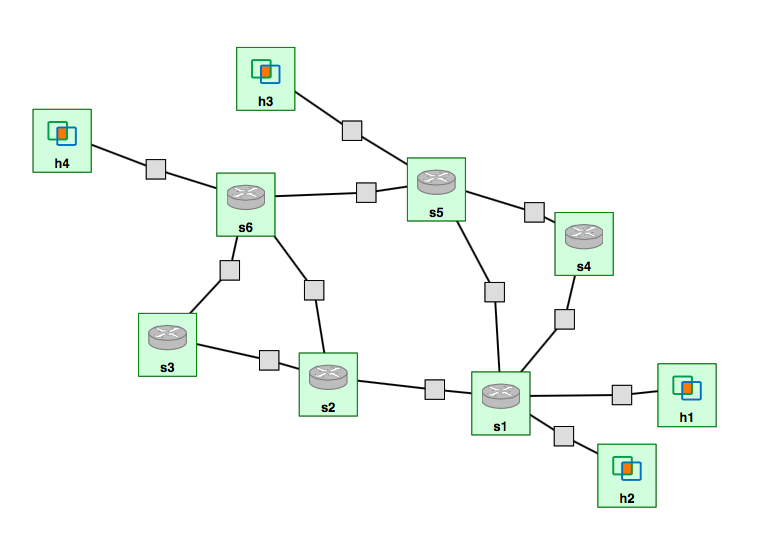
\includegraphics[scale=0.4]{topology.png}   
\end{center}
 \caption{GENI topology}
 \label{Fig 4.1}
\end{figure}
\begin{figure}[H]
\begin{center}
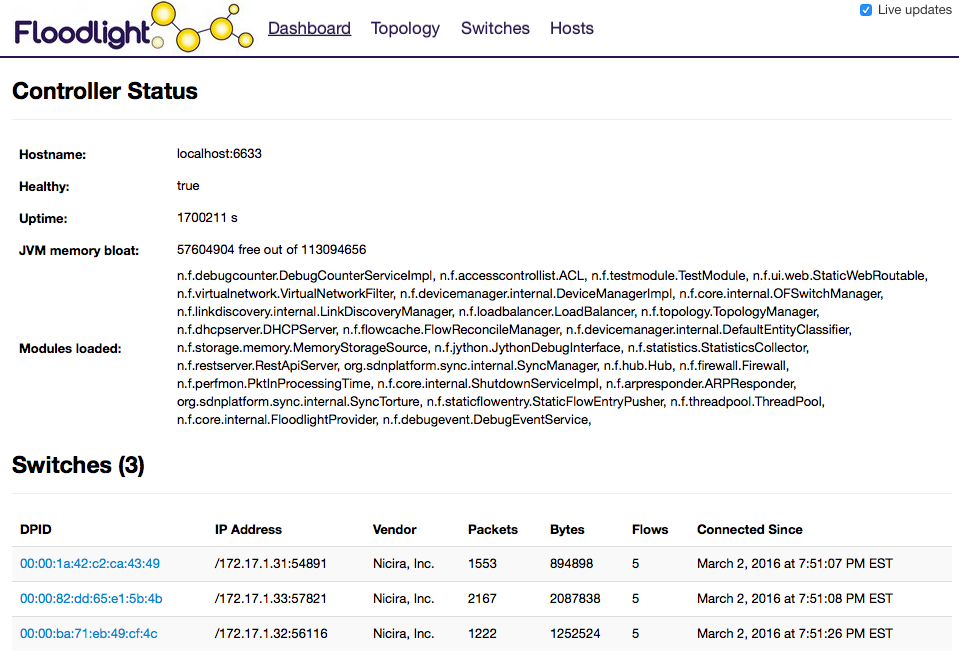
\includegraphics[scale=0.45]{floodlight.png}   
\end{center}
 \caption{Floodlight dashboard}
 \label{Fig 4.2}
\end{figure}
We can also see the OpenFlow rules that a switch is configured with in Figure \ref{Fig 4.3}. Right now, the rules shown are default shortest path rules that the floodlight controller pushed into the switches using the static flow pusher REST API.
\begin{figure}[H]
\begin{center}
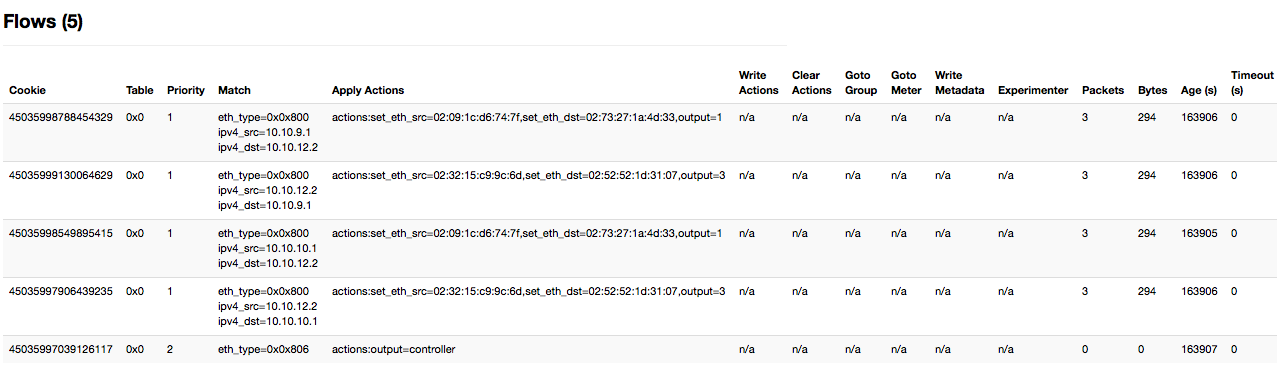
\includegraphics[scale=0.35]{rules.png}   
\end{center}
 \caption{Rule table in OpenFlow switch}
 \label{Fig 4.3}
\end{figure}
\subsection{Flow of the application}
The control flow of the application starts from constructing the network graph, polling the OpenFlow switches using the floodlight REST API to find active flows and then uses the statistics collector module of floodlight to query link statistics. Based on the statistics received, the application chooses a different path for active flows based on available link bandwidth.
\\
\\
The design decisions taken are the following:
\begin{itemize}
\item The topology is constructed using Python Networkx library undirected graph. The information for the nodes and the edges is received from the GENI RSpec document as well as the Floodlight controller REST API calls.
\item The bandwidth statistics from the statistics collector module of floodlight queries the links every 10 seconds.
\item The different simple paths are only on an end-to-end basis for a pair of hosts. A simple path means that no node is repeated in a path between two hosts.
\item A switch can only decide to change the path for a flow if the sender's IP is on the same subnet as the switch's interface.
\item The active flows are decided by polling the switches every 10 seconds and comparing the last packets hit count with the new polled information.
\item The application selects a different path based on aggregate available bandwidth from a list of simple paths between the source and the destination.
\item The aggregate available bandwidth for a path is actually the minimum available link bandwidth on the set of inter-switch links on that path.
\item The QoS rule written by the controller in the switches for a particular flow has an OpenFlow priority of `3' which makes sure that it receives precedence to any default shortest path rules for the same flow with priority `1'.

\end{itemize}

\subsubsection{Constructing the topology}
The application reads in the RSpec XML document from GENI portal and parses information about the names and interfaces of the nodes. The Python library used for parsing is "untangle" which converts XML to python objects. The node data items consist of the IP address, MAC address and port number for each of the interfaces connected to that node. The application then queries the controller using REST API commands to get respective OpenFlow Datapath ids (DPIDs) for the switches in the topology. Following command is used to get the DPID list from the controller:
\textit{
\begin{center}
"curl -s http://<controllerIp>/wm/core/controller/switches/json" 
\end{center}
}
To match a DPID received from the controller to the node name in GENI, the following REST API command is used:
\textit{
\begin{center}
"curl -s http://<controllerIp>/wm/core/switch/all/desc/json"
\end{center}
}
This command returns features of all the switches and the field 'datapathDescription' gives information to match the DPID to the node name from GENI.Similarly, the RSpec does not give information about the switch ports for the interfaces and the information about port numbers has to be queried from the controller using the following command:
\textit{
\begin{center}
"curl -s http://<controllerIp>/wm/core/switch/all/features/json"
\end{center}
}
For constructing the network graph after parsing the RSpec and querying the controller for the desired information, Python library "Networkx" is used which provides data structures for constructing network graphs. The library creates a Network object to which nodes and edges can be added. The nodes have the data items for interfaces as described above as well as the DPID and port numbers matched to the nodes using the controller information. 
\\
\\
Since the RSpec document or the controller do not provide information about the neighbors of the nodes or which interface is connected to which neighbor, the inter-host links are identified by matching the respective IP addresses in order to construct the edges between the nodes for the graph.

\subsubsection{Identifying hosts connected to the switches}
As mentioned in the design decisions, A switch can only decide to change the path for a flow if the sender's IP is on the same subnet as the switch's interface. To implement this, a structure 'switchHostsFlows' is constructed which specifies which hosts are on the switch subnet and which are the interfaces that connect to another switch instead of a host. It also specifies the possible source and destination pairs of a switch's traffic after polling all the shortest path flows in the OpenFlow table of that switch. This structure also maintains the flow statistics for each pair of source and destination hosts in the form of the last packet count. This information is later used to determine active flows in the network.
\\
\\
The hosts connected to the switch are identified by comparing the network address of interfaces of the hosts to the /24 network prefix of the interfaces of the particular switch. This structure only references the nodes which play the role of "hosts" on the network and not the ones which play the role of "switches".

\subsubsection{Enabling statistics collection}
In order to take advantage of the Floodlight controller statistics module REST API, it needs to be enabled in all the OpenFlow switches in the network. The command used to enable the statistics collection in the application is:
\textit{
\begin{center}
"curl -X POST -d ` ' http://< controllerIp>/wm/statistics/config/enable/json"
\end{center}
}
After statistics are enabled in the switches, the application can query the controller using the REST API commands specifying the switch using OpenFlow DPID and the desired port using the following command:
\textit{
\begin{center}
"curl http://<controllerIp>/wm/statistics/bandwidth/<switchDPID>/<port>/json"
\end{center}
}
The reply to the above command returns the transmission and reception bandwidth per switch per port in bits per second. The default interval when the bandwidth is reassessed by the controller is every 10 seconds \cite{stats}.
\subsubsection{Identifying inter-switch links}
The application also creates a list of links between the switches and the respective output switch ports for those links called the "interswitchLinks". This is important because the bandwidth calculation for paths is done solely on the basis of available bandwidth on the switch-switch links and not the switch-host links.
\subsubsection{Determine active flows}
As described in section 4.3.2, the structure "switchHostsFlows" keeps track of the last known packet count for a particular flow from a host to a destination. The application queries the controller to poll the switches for a list of flow statistics every 10 seconds using the command:
\textit{
\begin{center}
"curl -s http://<controllerIp>/wm/core/switch/<switchDPID>'/flow/json" 
\end{center}
}
For each shortest default path flow rule returned, the application checks if the source IP is from the same subnet as an interface from the switch DPID being polled by comparing to the list of switch hosts in 'switchHostsFlows'. If determined to be the gateway switch for that flow, the new packet count is compared to the stored last known packet count to determine if the flow is active. If a flow is found active, the function to calculate bandwidth for all alternate paths is called.

\subsubsection{Calculate available bandwidth for alternate paths}
The "calculate bandwidth for paths function" receives two arguments; a source and a target. The function calculates all simple paths between the source and the target using "all\_simple\_paths" method of the Python Networkx library. A simple path means that no node is repeated in a path between two hosts. If there is only one simple path returned, no alternate path is present between the two hosts i.e. only the shortest default path is available and the program returns to polling other active flows.
\\
\\
Using the information from the "interswitchLinks", the function uses the curl command from section 4.3.3 to get the transmission (TX) and reception bandwidth (RX) per switch per inter-switch port in bits per second. The TX and RX values are added to find the bandwidth usage in bits per second and then subtracted from the actual known link bandwidth to get available link bandwidth for each switch port and stored in a structure for using in path selection.
\\
\\
For each simple path calculated for a source-target pair, the function decides which switches and inter-switch ports are involved on that path. Using the stored bandwidth statistics, it calculates the available bandwidth for each path by finding the minimum available bandwidth for a link involved in that path.
\\
\\
After calculating available bandwidths on all paths, the function checks if any of the bandwidth values are better than the default shortest path. If yes, then it chooses the path with the best available value and returns the path. If not, then the function returns none and the flow remains on shortest path.

\subsubsection{Generate rule for path}
The "generate rule for path" function is called if the "calculate bandwidth for paths function" returns an alternate path for a pair of hosts. The function takes in three arguments; a path which is returned by the bandwidth function, a source IP and a destination IP. The function first checks the OpenFlow rule table of the switches involved in that path for a match of a priority `3' rule for the same source and destination IP using the following command.
\textit{
\begin{center}
"curl -s http://<controllerIp>/wm/staticflowpusher/list/<switchDPID>/json" 
\end{center}
}
If a rule already exists, the function returns and does not generate a new priority `3' rule. If no rule exists, the function determines the node and the next hop interface for each node in the path, finds the MAC address and switch port for forwarding and constructs a flow rule in JSON format to send via the static flow pusher REST API of Floodlight controller. A sample flow rule is shown in Figure \ref{Fig 4.4}. The command used by the application to push a generated flow through the controller to the switch is:
\textit{
\begin{center}
"curl -X POST -d `"+<JSON\_rule>+"' http://<controllerIp>/wm/staticflowpusher/json" 
\end{center}
}
\begin{figure}[H]
\begin{center}
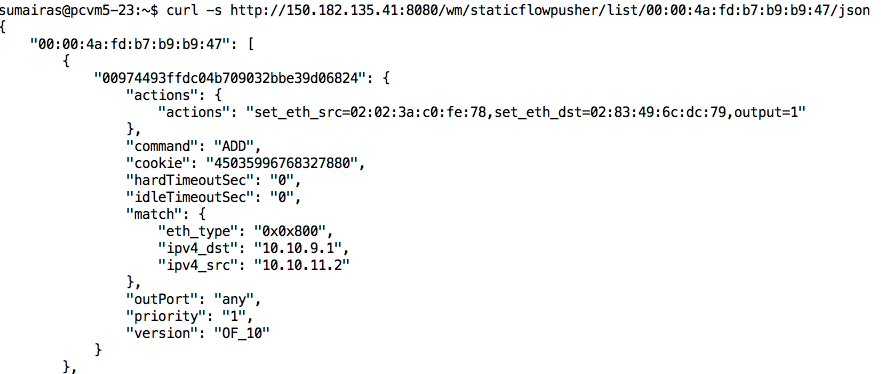
\includegraphics[scale=0.45]{flow.png}   
\end{center}
 \caption{A sample flow}
 \label{Fig 4.4}
\end{figure}
\section{Results}
\section{Challenges}
\section{Conclusion}
\bibliographystyle{ieeetr}% Select the citation style e.g. ieeetr
\bibliography{Smartgrid}% write the directory to the .bib file
%%% End document

\end{document}